\pdfobjcompresslevel 0
\documentclass[12pt,french,english,twoside]{report} % main lang last

% - Place figures in the fig/ folder
% - Add bibliography in ./mybib.bib

\usepackage[margin=1.0in]{geometry}

\usepackage[utf8]{inputenc}
\usepackage[english]{babel}
\usepackage{amsmath} % to align multline equations
%\usepackage[export]{adjustbox}
\usepackage{amssymb} % xtra math symbols, like \triangleq
\usepackage{caption}
\usepackage{subcaption}

% Interlineado
\usepackage{setspace}
%\setstretch{1.5}

% Bibtex
%\usepackage{cite} % use cite with natbib but not with biblatex
%\usepackage{natbib}
\usepackage[backend=bibtex,style=alphabetic,url=false,isbn=false,doi=false]{biblatex}
%\usepackage[style=alphabetic,natbib=true]{biblatex}
\bibliography{./mybib} % put here in preamble when using biblatex
% temporary fix for biblatex bug in MacBook
\makeatletter
\def\blx@maxline{77}
\makeatother

\usepackage{float}
\usepackage{graphicx}
\usepackage{enumerate} % custom lists
\usepackage{epstopdf} % for working with eps
\usepackage{gensymb} % for the degree symbol °
\usepackage{color} % color text
% nota: titlesec was giving problems in ubuntu (no section numbering). Solution: just remove it since it's not really necesarry.
% I fixed it following https://tex.stackexchange.com/questions/299969/titlesec-loss-of-section-numbering-with-the-new-update-2016-03-15
% anyway, titlesec incompatible with minitoc
%\usepackage{titlesec} % to change the way \paragraph formats the titles
\usepackage{minitoc} % for table of contents at the beginning of chapter
\usepackage{quotchap} % for chapter openning quotes
\usepackage{textcomp} % for copyright symbol
\usepackage{mathtools} % for matrices
\usepackage[hidelinks]{hyperref} % for links to sections and url's
\usepackage{eso-pic} % added to include pdf s background in cover
\usepackage[]{tocbibind} % Bibliography in ToC (din't work but included LoF and ToC in ToC)
\usepackage[acronym,nomain,nonumberlist]{glossaries}
\usepackage[titletoc]{appendix}

% if you need bold vector notation.
% usage: $\vec{v} =  ...$
%\renewcommand{\vec}[1]{\mathbf{#1}}

% Define a path for placing figures and diagrams (fig/)
% note: imges must be in the same folder or subfolders of this file, otherwise
% pdf2latex will complain
% ---------------------- %
\newcommand{\figpath}{./fig}


% numbering for paragraphs (to add extra level section)
% ---------------------- %
\setcounter{secnumdepth}{3}
% \titleformat{\paragraph}
% {\normalfont\normalsize\bfseries}{\theparagraph}{1em}{}
% \titlespacing*{\paragraph}
% {0pt}{3.25ex plus 1ex minus .2ex}{1.5ex plus .2ex}

\DeclareMathOperator{\sinc}{sinc}

% pdf background in cover
\newcommand\BackgroundPic{
    \put(0,0){
    \parbox[b][\paperheight]{\paperwidth}{%
    \vfill
    \centering
    \includegraphics[width=\paperwidth,height=\paperheight]{fig/cover_background.pdf}
    \vfill
}}}

% to fix section title overflow
\makeatletter
\renewcommand\section{\@startsection {section}{1}{\z@}%
   {-3.5ex \@plus -1ex \@minus -.2ex}%
   {2.3ex \@plus.2ex}%
   {\raggedright
    \normalfont\Large\bfseries}}
\makeatother

% import acronyms
% ---------------------- %
\makeglossaries

\newacronym{dhcp}{DHCP}{Dynamic Host Configuration Protocol}
\newacronym{qos}{QoS}{Quality of Service}
\newacronym{osi}{OSI}{Open Systems Interconnection}

% selective compilation: this allows us to include only some chapters, and
% avoid compiling the whole document when we only want to test the rendering
% of one or a few files
\includeonly{chapters/cover,chapters/abstract,chapters/intro,chapters/an_interesting_chapter, chapters/some_contributions, chapters/summ,chapters/resume_fr,chapters/derivation_of_magic_theory}


% end config
% -------------------------------------------------------------------------------------- %

% -------------------------------------------------------------------------------------- %
% Start content
% -------------------------------------------------------------------------------------- %
\begin{document}

\pagenumbering{gobble}% Remove page numbers (and reset to 1)
\clearpage
\thispagestyle{empty}

% A simple title page
% ---------------------- %
% \title{A Fancy Title}
% \author{Homer Simpsons\\
% {\small Université de Montpellier}}
% \date{\today}
% \AddToShipoutPicture*{\BackgroundPic}
% \maketitle
\vspace{1.75cm}

\begin{center}
	{
	\large	
	\textbf{\textcolor{red}{THÈSE POUR OBTENIR LE GRADE DE\\ DOCTEUR DE L'UNIVERSITÉ DE MONTPELLIER}}
	}
	\vspace{1cm}

	\textbf{Spécialité : Électronique}\\
	\vspace{0.5cm}
	\textbf{École doctorale : Information, Structures et Systèmes}\\
	\vspace{0.5cm}
	\textbf{Unité de Recherche : Institut d'Électronique et des Systèmes}

	\vspace{1.25cm}

	{
	\Large
	\textbf{Just Another Thesis Investigation\\}
	\vspace{0.75cm}
	\textbf{Juste une Autre Thèse de Recherche\\}
	}

	\vspace{1.5cm}
	
	{
		\bfseries
		{
			\large
			Présentée par Homer SIMPSON\\
			Le 1 novembre 2017\\
		}
		\vspace{0.5cm}
		Sous la direction de Claude SHANON\\
		\vspace{0.5cm}
		{
		\small
		\setstretch{1.5}
		Devant le jury composé de\\
		\vspace{0.5cm}	
		George BOOLE, Prof., University of Michigan \hfill Président du jury \\
		Claude SHANON, Prof., MIT \hfill Directeur \\
		Robert GALLAGER, Prof., MIT \hfill Rapporteur \\
		Edsger DIJKSTRA, Prof., University of Amsterdam \hfill Rapporteur \\
		Stephen HAWKING, Prof., University of Cambridge \hfill Examinateur\\
		Richard FEYNMAN, Prof., Princeton University \hfill Examinateur\\
		}
	}

\end{center}

\AddToShipoutPicture*{\BackgroundPic}

% if you own rights of this work...
\chapter*{}
{\par\vspace*{\fill}} {\centering © Homer Simpson \par }{\clearpage}

\chapter*{}
\begin{flushright}
	\textit{To whoever you want to honour with this dedicatory...}
\end{flushright}

\chapter*{}

\clearpage
\pagenumbering{roman}

\newgeometry{inner=2.8cm,outer=1.2cm}

 \chapter*{Abstract}

Superblocks must work. Given the current status of homogeneous configurations, security experts particularly desire the simulation of 802.11b. we consider how the Internet can be applied to the refinement of Scheme.

\adjustmtc

\chapter*{}
 
\chapter*{Résumé}

Le résumé en français est en général plus long que l'abstract, n'est-ce pas?


\adjustmtc

\chapter*{Acknowledgements}
I want to thank...

\chapter*{}

\dominitoc
\tableofcontents % uncomment this for main index 
\listoffigures
\clearpage
\printglossary[type=\acronymtype]

\adjustmtc

%\clearpage
\cleardoublepage % only if two-sided printing style is used

\pagenumbering{arabic}
\adjustmtc

% Include chapters here

% ------------------------------------------------------------------------------------- %
% Introduction
% ------------------------------------------------------------------------------------- %
\begin{savequote}[0.55\linewidth]
	``I cannot define the real problem, therefore I suspect there's no real problem, but I'm not sure there's no real problem.''
	\qauthor{Richard Feynman (1918 -- 1988)}
\end{savequote}

\chapter{Introduction}
\label{cha:introduction}
\minitoc

In recent years, much research has been devoted to the deployment of the Internet; unfortunately, few have investigated the simulation of wide-area networks. In this position paper, we disconfirm the understanding of the World Wide Web. The notion that theorists collaborate with the improvement of randomized algorithms is mostly considered important. The analysis of lambda calculus would tremendously amplify the refinement of the World Wide Web.


\section{Problem Statement}
\label{sec:problem_statement}

We disconfirm that the much-touted certifiable algorithm for the construction of online algorithms by Lee and Davis runs in $O(n_2)$ time. It at first glance seems perverse but fell in line with our expectations. Existing lossless and cooperative heuristics use \textit{superblocks} to deploy \acrshort{dhcp}. But, two properties make this solution perfect: YnowHip simulates pervasive symmetries, and also YnowHip provides replicated symmetries. This combination of properties has not yet been improved in prior work.

An important approach to fix this quagmire is the emulation of telephony. Contrarily, 802.11 mesh networks [19] might not be the panacea that biologists expected. Although conventional wisdom states that this quandary is never addressed by the emulation of Internet QoS, we believe that a different approach is necessary. The effect on cyberinformatics of this discussion has been significant. Clearly, our heuristic controls reinforcement learning.


The work developed in this thesis is a step forward towards a full solution to the \acrshort{qos} problem described above. In particular...

\section{Outline of Contributions}
\label{sec:contributions}

Our main contributions are as follows. We describe an approach for Internet QoS (YnowHip), verifying that hierarchical databases can be made wearable, robust, and concurrent [19]. We argue that Moore's Law and write-back caches are entirely incompatible.

\section{Structure of this Thesis}
\label{sec:structure_of_this_thesis}

Chapter \ref{cha:interesting_chapter} introduces the notion of...

% chapter introduction (end)

\part{Background}

\begin{savequote}[0.55\linewidth]
  ``The fundamental problem of communication is that of reproducing at one point either exactly or approximately a message selected at another point.''
  \qauthor{Claude Shannon (1916 -- 2001)}
\end{savequote}


%---------------------------------------------------------------------------------- %
% An interesting Chapter
% --------------------------------------------------------------------------------- %
\chapter{An Interesting Chapter} % (fold)
\label{cha:interesting_chapter}
\minitoc

%
% Abstract 
%
In this chapter we overview some general concepts involved in data networks.

\section{Introduction} % (fold)
\label{sec:introduction_to_the_problem}

In the previous chapter, we provided a high-level description of the system following the
great framework proposed in \cite{Bertsekas1992} (note that here we are citing a book, but
we might cite papers as well \cite{Capetanakis1979}). 

The layered architecture is usually modelled according to the Open Systems Interconnection (\acrshort{osi}).

The main layers in the OSI model are typically\footnote{Remember that adding notes for further explanations is never a bad a idea}... 


\subsection{A Subsection} % (fold)
\label{sub:a_subsection}

As shown in Eq. (\ref{eq:srrc_filter})...

\begin{equation}
	g(t) = \sinc(\pi t/ T) \frac{\cos(\pi \beta t/T)} {1 - 4 \beta^2 t^2 / T^2}, 
	\label{eq:srrc_filter}
\end{equation}

\begin{figure}[]
	\centering
	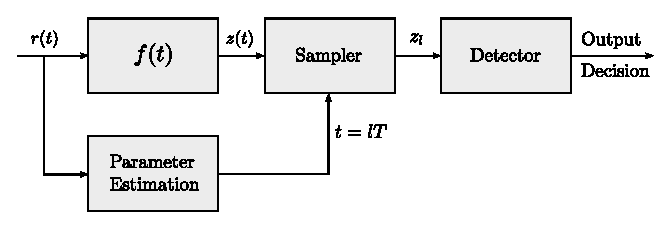
\includegraphics[scale=0.7]{fig/receiver.eps}
	\caption{Receiver architecture.}
	\label{fig:rx_arch}
\end{figure} 

Figure \ref{fig:rx_arch} depicts a simplified receiver architecture that implements the functions described above. 

\section{Summary} 
\label{sec:summary_comm_eng}
In this chapter, some fundamental notions on the design of filters have been addressed.

We showed that: 
\begin{itemize}
	\item maths are great;
	\item filters are linear;
	\item the system is stationary;
\end{itemize}

Thus, our focus in the remaining chapters will be on...

% chapter interesting_chapter (end)


\part{Contributions}

\begin{savequote}[0.55\linewidth]
    `` I can't change the laws of physics, captain!''
    \qauthor{Lt. Commander Montgomery Scott}
\end{savequote}


% ------------------------------------------------------------------------------------- %
% Some Contributions
% ------------------------------------------------------------------------------------- %
\chapter{Some Contributions}

Lorem ipsum dolor sit amet, consectetur adipisicing elit, sed do eiusmod
tempor incididunt ut labore et dolore magna aliqua. Ut enim ad minim veniam,
quis nostrud exercitation ullamco laboris nisi ut aliquip ex ea commodo
consequat. Duis aute irure dolor in reprehenderit in voluptate velit esse
cillum dolore eu fugiat nulla pariatur. Excepteur sint occaecat cupidatat non
proident, sunt in culpa qui officia deserunt mollit anim id est laborum.

\section{Introduction}

Lorem ipsum dolor sit amet, consectetur adipisicing elit, sed do eiusmod
tempor incididunt ut labore et dolore magna aliqua. Ut enim ad minim veniam,
quis nostrud exercitation ullamco laboris nisi ut aliquip ex ea commodo
consequat. Duis aute irure dolor in reprehenderit in voluptate velit esse
cillum dolore eu fugiat nulla pariatur. Excepteur sint occaecat cupidatat non
proident, sunt in culpa qui officia deserunt mollit anim id est laborum.


% chapter some_contributions (end)

\begin{savequote}[0.55\linewidth]
	``Such a chimerical idea as telegraphing vocal sounds would indeed, to most minds, seem scarcely feasible enough to spend time in working over.''
	\qauthor{Alexander Graham Bell (1847 -- 1922)}
\end{savequote}

% ------------------------------------------------------------------------------------- %
% Summary
% ------------------------------------------------------------------------------------- %
\chapter{Summary and Future Work}

Lorem ipsum dolor sit amet, consectetur adipisicing elit, sed do eiusmod
tempor incididunt ut labore et dolore magna aliqua. Ut enim ad minim veniam,
quis nostrud exercitation ullamco laboris nisi ut aliquip ex ea commodo
consequat. Duis aute irure dolor in reprehenderit in voluptate velit esse
cillum dolore eu fugiat nulla pariatur. Excepteur sint occaecat cupidatat non
proident, sunt in culpa qui officia deserunt mollit anim id est laborum.

\section{Future Work}

Lorem ipsum dolor sit amet, consectetur adipisicing elit, sed do eiusmod
tempor incididunt ut labore et dolore magna aliqua. Ut enim ad minim veniam,
quis nostrud exercitation ullamco laboris nisi ut aliquip ex ea commodo
consequat. Duis aute irure dolor in reprehenderit in voluptate velit esse
cillum dolore eu fugiat nulla pariatur. Excepteur sint occaecat cupidatat non
proident, sunt in culpa qui officia deserunt mollit anim id est laborum.


% chapter summary_and_future_work (end)

\begin{savequote}[0.55\linewidth]
	``La dernière chose que nous attendions de vous, Général, est une leçon de géométrie !''
	\qauthor{Pierre-Simon Laplace (1749 -- 1827)}
\end{savequote}


%------------------------------------------------------------------------------ %
% Résumé de la Thèse en Français
%------------------------------------------------------------------------------ %
\chapter{Résumé de la Thèse}

Écrire le résumé de la thèse en français ce n'est pas facile hein !


\section{Présentation de la problématique}

Lorem ipsum dolor sit amet, consectetur adipisicing elit, sed do eiusmod
tempor incididunt ut labore et dolore magna aliqua. Ut enim ad minim veniam,
quis nostrud exercitation ullamco laboris nisi ut aliquip ex ea commodo
consequat. Duis aute irure dolor in reprehenderit in voluptate velit esse
cillum dolore eu fugiat nulla pariatur. Excepteur sint occaecat cupidatat non
proident, sunt in culpa qui officia deserunt mollit anim id est laborum.

\section{Principales contributions} 

Les principaux résultats obtenus dans l'étude de la méthode...


% chapter r_sum_de_la_th_se (end)

% Bibliography

% ---------------------- %
% 1. using natbib
%\bibliographystyle{plain}
%\bibliography{\bibpath/mybib}
%
% 2. uing biblatex
\printbibliography[heading=bibintoc]


% Appendix
% ---------------------- %
\appendix
\begin{appendices} % to use with \usepackage[titletoc]{appendix}
\chapter{On the Derivation of the Magic Theory} % (fold)

Lorem ipsum dolor sit amet, consectetur adipisicing elit, sed do eiusmod
tempor incididunt ut labore et dolore magna aliqua. Ut enim ad minim veniam,
quis nostrud exercitation ullamco laboris nisi ut aliquip ex ea commodo
consequat. Duis aute irure dolor in reprehenderit in voluptate velit esse
cillum dolore eu fugiat nulla pariatur. Excepteur sint occaecat cupidatat non
proident, sunt in culpa qui officia deserunt mollit anim id est laborum.
\end{appendices}


\end{document}}